
% Section: ARCHITECTURE

\section{Architecture for Community Network Cloud}
%\subsection{Framework for Distributed Community Cloud System}
\label{sec__cloud_arch}

%% >> Updated text copied from ComNet'15 paper
We foresee realising the community cloud by deploying a community cloud platform tailored to the specific infrastructure and context of community networks. 
A standard cloud system is usually a centralised platform designed to perform resource management. 
There are quite a few well known cloud platforms for managing public and private clouds, 
like OpenStack~\cite{OpenStack} and OpenNebula~\cite{OpenNebula} among others. 
For community network cloud, we focus on providing a framework that would allow users to share resources and access collaboratively-built services in a distributed manner.
%For instance, a community cloud platform would require incentive mechanisms inspired by the social nature of community networks integrated into resource regulation components to encourage contribution from the members of the community network~\cite{Khan2015Incentive}.

%\subsection{Layers of Community Cloud System}
We propose a framework that can serve as the core of a community cloud system. 
Our community cloud framework is a distributed bottom-up resource sharing and collaborative services platform.
This is achieved by adopting a layered architecture, as shown in Figure~\ref{fig:cloud-architecture}. 

\begin{figure}[tbp]
	\centering
	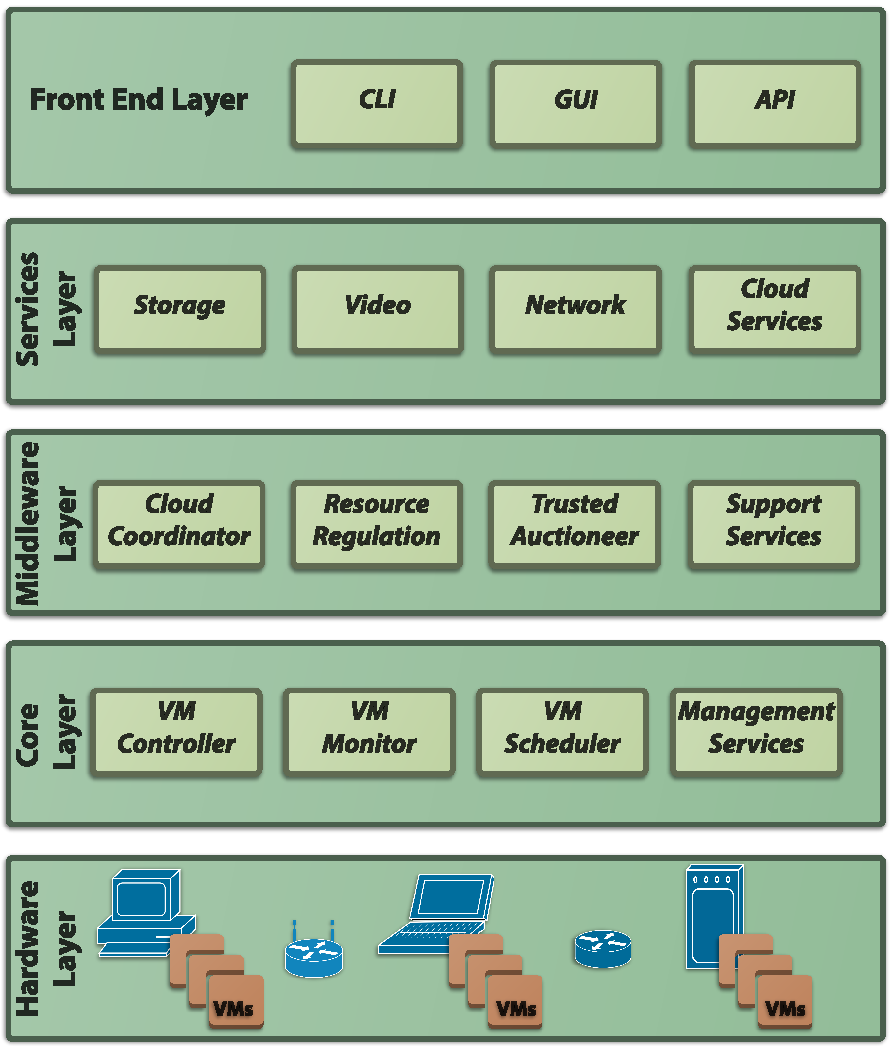
\includegraphics[width=0.75\textwidth,keepaspectratio]{architecture} 
	\caption{Framework for community cloud management system}
	\label{fig:cloud-architecture}
\end{figure}

\begin{enumerate}
	
	\item The \textbf{Hardware layer} provides the physical infrastructure needed to run the cloud services and applications. 
	The hardware in the community network customarily consists of management nodes, 
	client nodes, routers and the communication infrastructure, 
	along with any computation, storage and other resources attached to the nodes.
	
	\item The \textbf{Core layer} is responsible for managing the hardware as virtualised resources. 
	It consists of components, such as a manager for the hosts and the network 
	as well as a controller, scheduler, monitor, and data storage for virtual machines (VMs). 
%	Many popular open-source software programs can be integrated to provide virtualisation, for instance 
%		LXC (Linux Containers)~\cite{LXC}, 
%		OpenVZ~\cite{OpenVZ}, 
%		and Docker~\cite{Docker}, etc.

	\item The \textbf{Middleware layer} amalgamates the resources from multiple local community clouds, providing an integrated and consistent view of the cloud system to the cloud services. 
	This can comprise of a variety of support services:

	\begin{itemize}

		\item \textbf{Cloud coordinator} and services broker components for assisting in combining resources from multiple cloud providers.

		\item Incentives-based \textbf{resource regulation} and allocation components 
		are important as a driver for users' participation 
		for the sustainability and growth of the community cloud model.
		Our proposed incentive mechanisms in \Cref{chap__incentives} can provide the building blocks for these components.

		\item \textbf{Trusted auctioneer} module for auction-based resource allocation schemes. % ~\cite{Khan2016Distributed}
		Resource allocation component needs to be trusted by the users,
		and in turn the users need to follow the prescribed polices for the system to function properly.
		We return to this issue in \Cref{chap__trusted_auction}, and devise a virtual distributed trusted auctioneer
		to integrate into the community cloud framework.

		\item Other \textbf{support services} may include, among many other:
		
		\begin{itemize}
			\item Network coordination component to identify and manage different local clouds.
			\item Service discovery component to keep track of the services provided by the various clouds.
			\item Authentications and auditing components to support resource regulation.
		\end{itemize}

	\end{itemize}

	\item The \textbf{Services layer} integrates useful services and applications providing utilities for the community network members to encourage their participation. 
	Common services include storage, video streaming, video on demand, IP telephony, and network applications.

	\item The \textbf{Front-end layer} provides the interface to interact with the infrastructure of the community cloud, including
		command line interfaces (CLI), 
		graphical user interfaces (GUI), 
		application programming interfaces (API), 
	and any other tools for assisting in the development of cloud services and applications.

\end{enumerate}

%
%\subsection{Resource Regulation}
%
%
%\subsection{Trusted Auctioneer}

